%----------------------------------------------------------------------------------------
%       CHAPTER 8
%----------------------------------------------------------------------------------------

\cleardoublepage

\chapterimage{origin.jpg} % Chapter heading image

\chapter{The geological cycle of carbon}\label{ch:geological-carbon}

\hfill \break

\vspace{24mm}

\noindent

%------------------------------------------------
\newpage
%------------------------------------------------

\section*{README}

You will need to download a new \textit{re-start} file. To fetch this -- change to the \textsf{\footnotesize cgenie\_output directory}, and type:
\vspace{-1mm}\small\begin{verbatim}
$ wget --no-check-certificate http://www.seao2.info/cgenie_output/ ...
231228.muffin.CBSR.fkl_pp51.BASESw.SPIN2.tar.gz
\end{verbatim}\normalsize\vspace{-1mm}
\noindent Extract the contents of this archive by typing:
\vspace{-1mm}\small\begin{verbatim}
$ tar xfzv 231228.muffin.CBSR.fkl_pp51.BASESw.SPIN2.tar.gz
\end{verbatim}\normalsize\vspace{-1mm}
You’ll then need to change directory back to \textsf{\footnotesize genie-main } directory in order to run \textbf{muffin}.

%------------------------------------------------
\newpage
%------------------------------------------------

\section{The long tail of CO$_{2}$ (and other tales from the sediments)}

This chapter introduces the marine sediment model component in muffin -- \textbf{SEDGEM} (SEDiment GEochemistry Model) plus \textbf{ROKGEM}, the terrestrial weathering module. In terms of the fate of fossil fuel \(CO_{2}\), the model configuration and experiments in this chapter include: a representation of deep-sea sediments and the interaction between the preservation and burial of \(CaCO_{3}\) and ocean chemistry plus, plus the balance (or imbalance) between weathering on land and sedimentary burial (of \(CaCO_{3}\)) (all in addition to the interaction between atmosphere and ocean and redistribution of carbon within the ocean as previously). For an over-view of the sediment model and what time-scales and nature of carbon cycle interaction between ocean and sediment you can expect, read: \textit{Ridgwell and Zeebe} [2005] and \textit{Ridgwell and Hargreaves} [2007]. \textbf{ROKGEM} is described in \textit{Colbourn et al.} [2013].

Beyond the basic 'inorganic' geological carbon cycle\footnote{As per described in the references above.}, also included are:

\begin{itemize}[noitemsep]
\setlength{\itemindent}{.2in}
\item Weathering of rock-hosted organic carbon (kerogens).
\item Weathering of phosphorous (e.g. from apatite).
\item Burial of organic carbon (as a function of flu to the sediment surface).
\item Differential regeneration and return of dissolved phosphorous back to the ocean (as a function of dissolved oxygen concentrations in bottom waters).
\end{itemize}

All these processes and feedbacks can be 'fixed' (made invariant) or disabled to test their importance (or not) in the long-term regulation of atmospheric \(pCO_{2}\) and climate dynamics and in comparison with published analyses based only on the 'inorganic' carbon cycle (and silicate weathering as the only long-term feedback on atmospheric \(pCO_{2}\)).

\begin{figure}
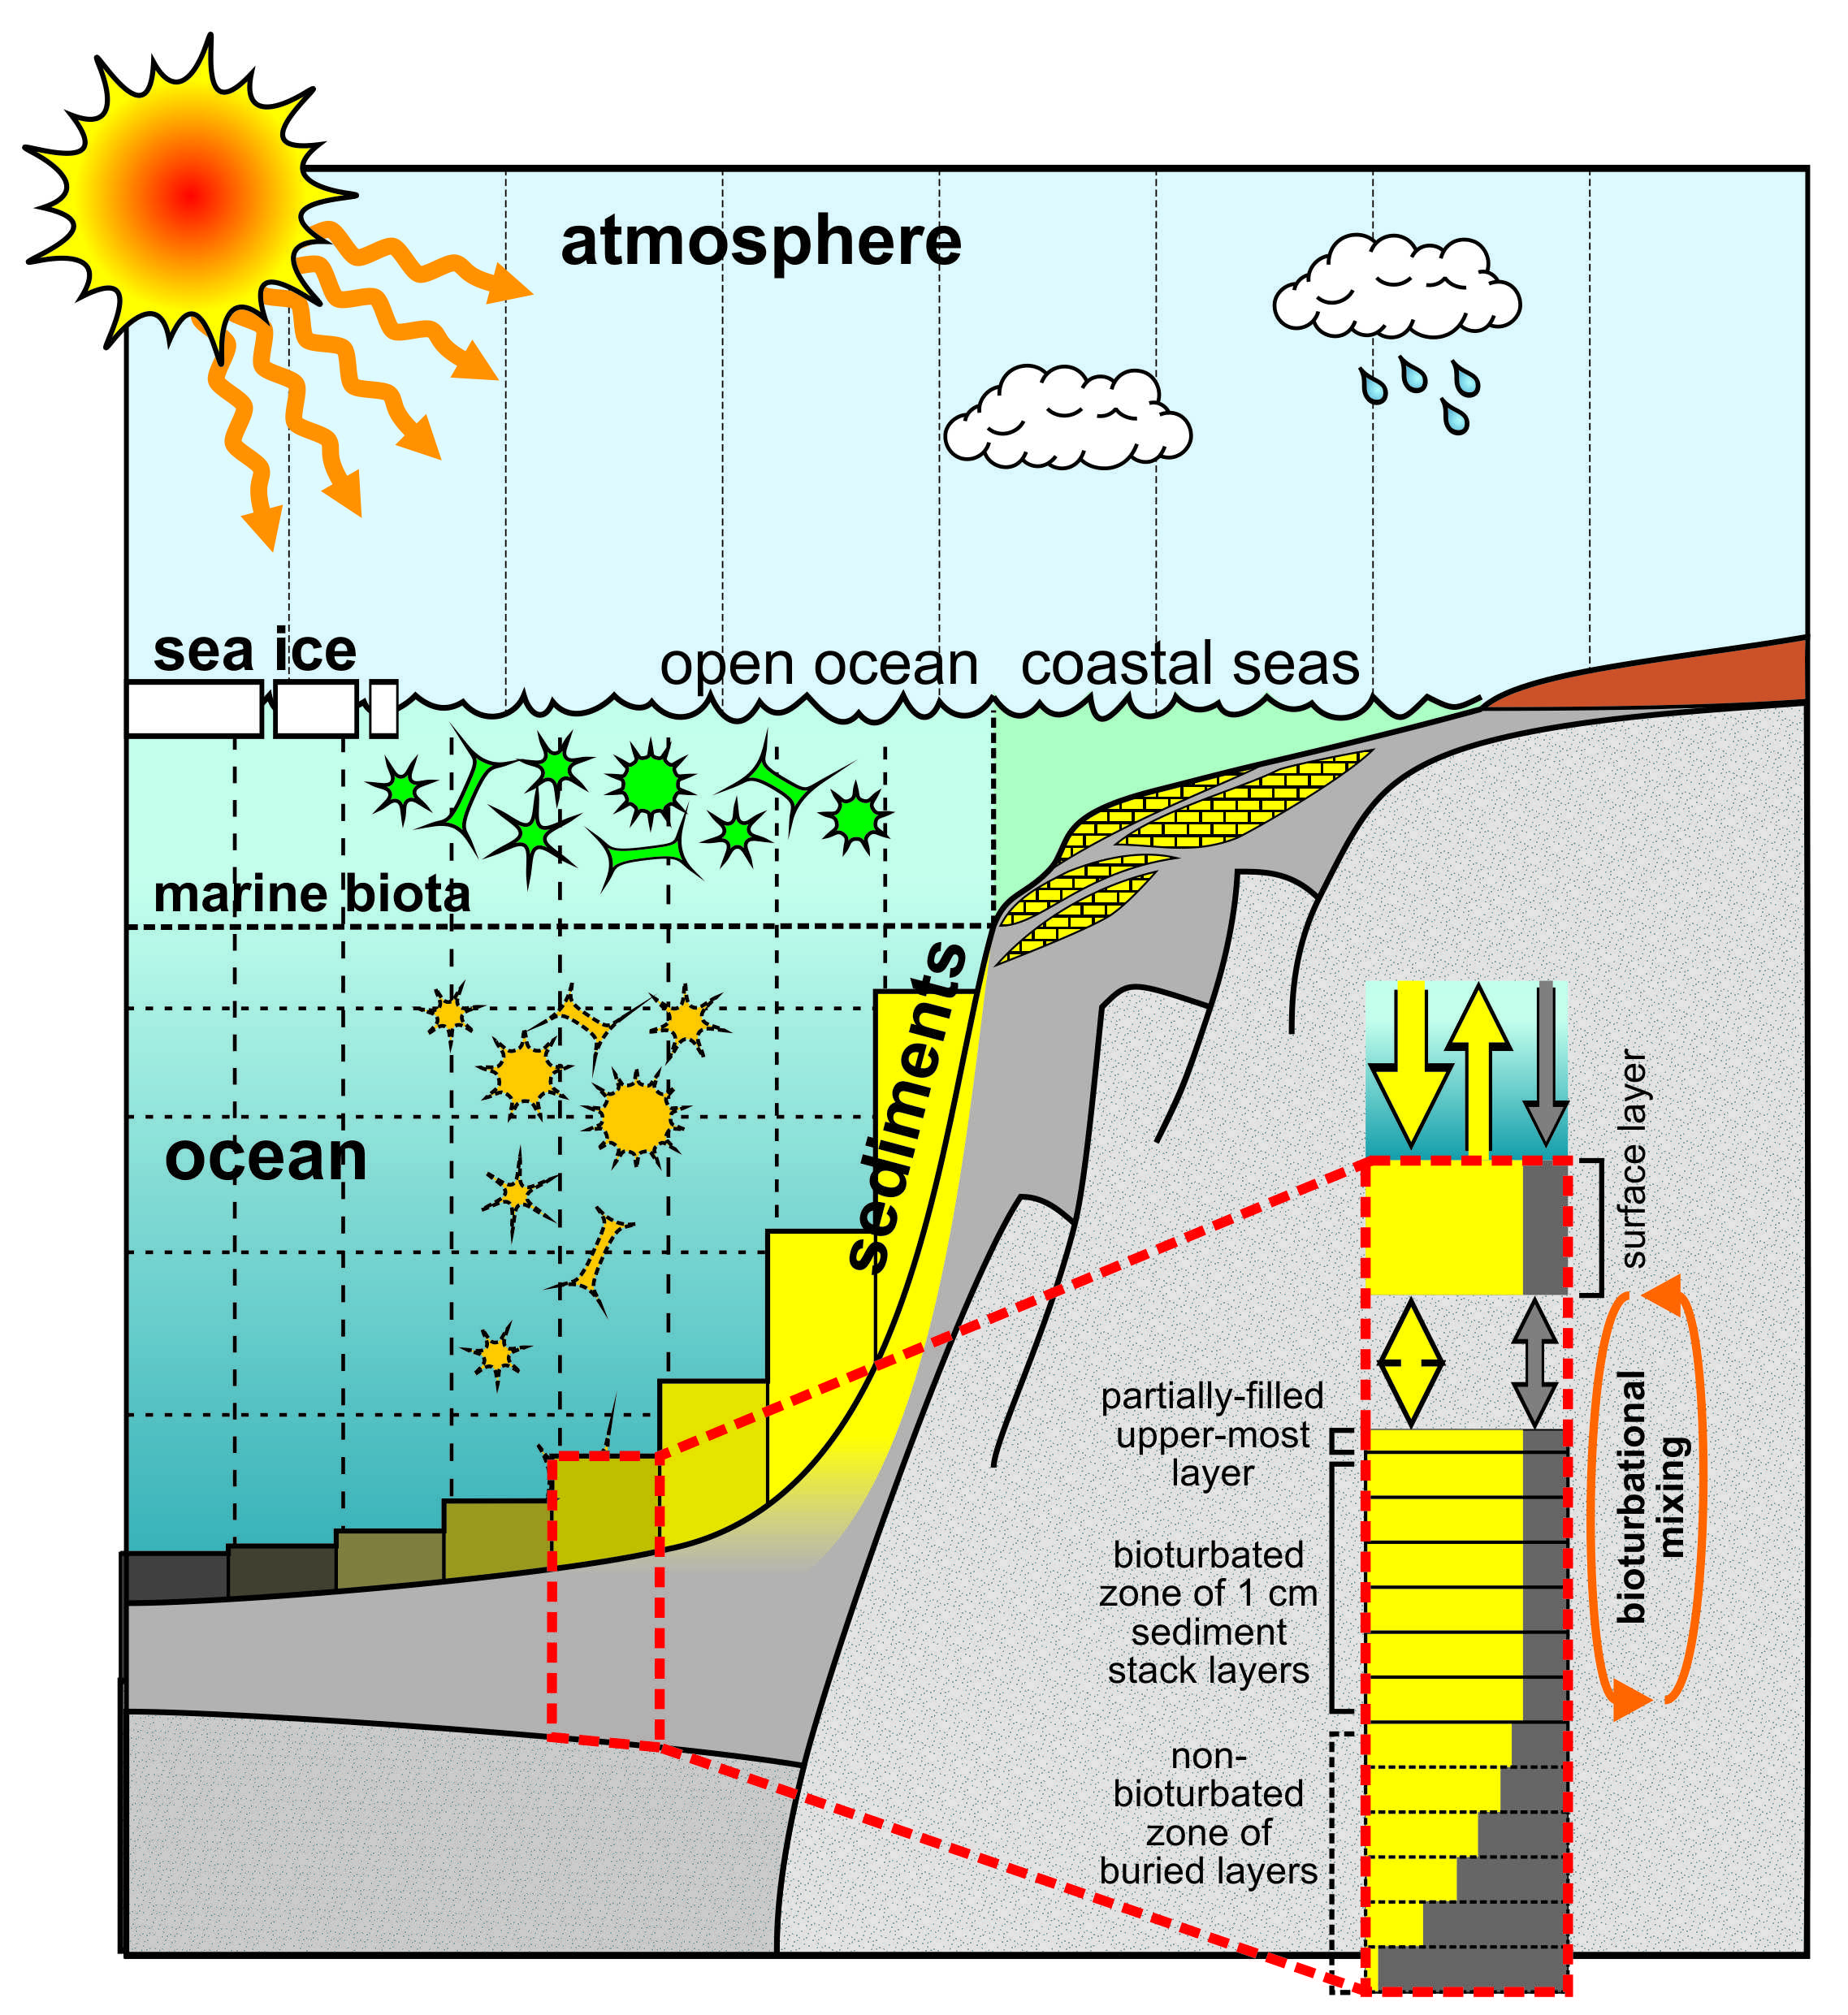
\includegraphics[width=0.5\textwidth]{sediments.jpg}
\caption{Schematic of \textbf{SEDGEM} sediment component.}
\label{fig:sediments}
\end{figure}

%------------------------------------------------
\vspace{1mm}
\noindent\rule{4cm}{0.1mm}
\vspace{2mm}
%------------------------------------------------

%------------------------------------------------
\newpage
%------------------------------------------------

\noindent Take the new model configuration for a test drive by running on from the \textit{re-start} experiment that you downloaded.

This is a steady-state climate+carbon cycle experiment that includes the deposition of \(CaCO_{3}\) in deep-sea sediments as well as the deposition of organic matter on continental shelves (plus a more minor contribution in deep-sea sediments), balanced by weathering (solute input to the ocean) plus volcanic \(CO_{2}\) out-gassing ... or at least as closely in balance as possible after 50,000 years. Try running ('briefly', but 100 years would not be too tedious for this faster configuration!) the following:

\vspace{-2mm}\small\begin{verbatim}
$ ./runmuffin.sh muffin.CBSR.fkl_pp51.BASESw
 LABS ch09.1.CTRL 100 231228.muffin.CBSR.fkl_pp51.BASESw.SPIN2
\end{verbatim}\normalsize\vspace{-2mm}

The \textit{user-config} \textsf{\footnotesize ch09.1.CTRL} is set up with the global carbon cycle configured as 'open' -- that is to say, that there is an input of carbon, alkalinity, and phosphorous to the ocean from weathering (plus carbon from volcanic out-gassing), and a loss due to preservation and burial of \(CaCO_{3}\) and organic matter in marine sediments. Depending on the state of ocean chemistry (and biology) and weathering, these two fluxes (input vs. output) do not have to balance, and hence ocean carbonate chemistry (and in turn, atmospheric \(pCO_{2}\)) can evolve with time. The \textit{spin-up} may not necessarily have the input and output fluxes absolutely perfectly balanced and hence before you run any experiments you might want to confirm whether the spin-up provided really is adequately 'spun-up'\footnote{i.e., you might plot some of the variables from the results of the \textit{spin-up}  experiment as a function of time and judge whether they are sufficiently converged or not.}. \textsf{\footnotesize ch09.1.CTRL} is hence configured to act as a control and quantify any residual flux imbalance and hence geochemical)(and climatic) 'drift'.

Note that a residual drift can be dealt with if it is relatively small and near linear via the use of a \uline{control experiment}, because any experiment you carry out will likely also incorporate (or be biased) by the same residual drift. Running a control gives you something to directly contrast  your experiment with and calculating the difference (e.g., a difference map or simple subtraction of global numbers) will give you the effect of whatever parameters you changed in the experiment but corrected for any drift. In previous exercises, you may have been a little lazy and created difference maps with respect to year 1 of an experiment -- strictly, they should have been created relative to the same year of a parallel control experiment, e.g., the results of a perturbation after 100 years should be contrasted with the year 100 results of the equivalent control.

%------------------------------------------------
\newpage
%------------------------------------------------

\noindent Before you look at any output from this experiment, you should note the following about this particular configuration and experiment:

\begin{enumerate}[noitemsep]
\vspace{1mm}
\item In the \textit{base-config} file naming convention -- the the '\textsf{\footnotesize S}' in \textsf{\footnotesize muffin.CBSR.fkl\_pp51.BASESw} specifies the use of a sediment model and the '\textsf{\footnotesize R}' a weathering module (see references should should have only just read!)\footnote{In addition to ocean and atmosphere biogeochemistry -- '\textsf{\footnotesize B}' and climate components (ocean, sea-ice, EMBM atmosphere) -- '\textsf{\footnotesize C}'.}
\vspace{1mm}
\item The '\textsf{\footnotesize w}' in \textsf{\footnotesize BASESw} specifies that a 'weathering' tracer has been included, which for simplicity, is dissolved silica. (See discussion later.)
\vspace{1mm}
\item We are running at a degraded (lower) \(18\times18\) resolution (but still \(16\) vertical levels in the ocean), and requiring fewer (twice as few in fact!) time-steps per year, for an overall approximately order-of-magnitude decrease in run-time as compared to a more standard \(36\times36\) resolution configuration of \textbf{muffin}. This is extremely helpful in being able to run \textbf{muffin} on geological time-scales but within a reasonable about of real time.
\vspace{1mm}
\item The configuration utilizes a conceptual/idealized continental configuration somewhat similar to as in the snowball Earth experiments.
\vspace{1mm}
\item Although this configuration could be regarded as a maximum complexity system, we are only going to initially look at this from the perspective of new output, and will reduce the complexity right down before we start to think about system behavior.
\vspace{1mm}
\item Data saving is set up for 2D only in \textbf{BIOGEM} (and not 3D), \textit{time-slices} only every 10000 years, and \textit{time-series} save points only every 100 years (all to minimize the size of the results files for loooooong experiment durations):
\vspace{-1mm}\small\begin{verbatim}
# force time-series saving @ 100 yr intervals
bg_par_infile_sig_name='save_timeseries_EVERY000100.dat'
# force 2D time-slice save only, and @ 10000 yr intervals
bg_ctrl_data_save_2d=.true.
bg_ctrl_data_save_3d=.false.
bg_par_infile_slice_name='save_timeslice_EVERY010000.dat'
\end{verbatim}\normalsize\vspace{-1mm}
You can return to the default saving you are used to by commenting out all these lines. Or you could change the name of the \textit{time-slice} and \textit{time-series} saving interval files, but making sure first the new file name exists (in directory: \textsf{\footnotesize genie-biogem/data/input} OR creating your own file there (and using that name).
\\Note that although a 100 year experiment will not yet have reached the first save point (with a mid-point time of 9999.5 years), \textbf{muffin} is configured to ALWAYS save you a final year \textit{time-slice}, regardless of whether your experiment duration ends up reaching a specific save point at run-end or not.
\vspace{1mm}
\item To date, the marine biochemical cycle of carbon and nutrients in muffin has included an 'implicit' alkalinity contribution (see Section 2.1 in: \textit{Ridgwell et al.} [2007]). In a fully open system with weathering and burial or organic carbon and nutrients, this becomes invalid. hence the inclusion in the \textit{user-config} of:
\vspace{-1mm}\small\begin{verbatim}
# *** BIOGEM ********************************************************
# remove organic matter associated (implicit nitrogen) alkalinity transformations
# => so we do not end up with spurious weathering ALK fluxes from kerogens 
#    (or spurious Corg burial related fluxes)
bg_par_bio_red_PON_ALK=0.0
\end{verbatim}\normalsize\vspace{-1mm}
%------------------------------------------------
\newpage
%------------------------------------------------
and in diagnosing \textbf{ROKGEM} parameter values:
\vspace{-1mm}\small\begin{verbatim}
# *** SEDGEM configuration ******************************************
# weathering diagnostic settings    
sg_par_sed_diag_P2ALK=0.0
\end{verbatim}\normalsize\vspace{-1mm}
\vspace{1mm}
\item Before we move on, a final instructive change from previously published configurations is:
\vspace{-1mm}\small\begin{verbatim}
# *** ROKGEM ********************************************************
# turn off atmospheric short circuit 
# (so CO2 is now removed from the atmosphere during weathering, 
#  and volcanic CO2 added to it)
# => to better diagnose weathering in BIOGEM output
rg_opt_short_circuit_atm=.false.
\end{verbatim}\normalsize\vspace{-1mm}
During weathering (of carbonate and silicate rocks), \(CO_{2}\) is assumed to dissolve in rainwater and reach with the calcium-bearing minerals. Later, in the ocean, when \(CaCO_{3}\) is precipitated and \(CO_{2}\) 'released'\footnote{Technically: made available for exchange with the atmosphere by a shift to lower pH.}, the \(CO_{2}\) originally removed from the atmosphere is regenerated/replaced. The 'short-circuit' is simple to assume this and not bother removing the one mol of \(CO_{2}\) in reaction with a mol of \(CaCO_{3}\) or \(CaSiO_{3}\). The \(CO_{2}\) consumption and removal from the atmosphere associated with silicate weathering is also not removed, on the basis that the alkalinity transported by rivers and added to the ocean will drive the draw-down if atmospheric \(pCO_{2}\) at that stage (rather than being removed up-front). Hence, in short-circuiting, the DIC transported to the ocean in rivers is equal to the weathering flux of carbon in \(CaCO_{3}\) plus the rate of \(CO_{2}\) out-gassing.

However, this only really 'works' if the system is in some sort of balance of weathering and precipitation and that alkalinity added to the surface ocean can fully equilibriate with the atmosphere ... which will not be the case during transient events (see Figure 3 in: \textit{Lord et al.} [2015]). Setting: \textsf{\footnotesize rg\_opt\_short\_circuit\_atm=.false.} instead tracks the \(CO_{2}\) fluxes explicitly and in full.
\\The potential implications of this will be a subject of a subsequent investigation ...
\\NOTE: A 'short-circuit' is fine if you are only looking at long-term weathering vs. sedimentation steady-states and not rapid carbon release driven transients.
\end{enumerate}

\vspace{1mm}
\noindent Other parameter settings will be introduced and explained as and when needed during this chapter.

%------------------------------------------------
\vspace{1mm}
\noindent\rule{4cm}{0.1mm}
\vspace{2mm}
%------------------------------------------------

%------------------------------------------------
\newpage
%------------------------------------------------

\section{Sediment model output}

There is a whole new set of additional outputs from this configuration of \textbf{muffin}, particularly sediment-specific output from the \textbf{SEDGEM} module and which is saved in the \textsf{\footnotesize sedgem} sub-directory of the main experiments results directory. Data saving differs from \textbf{BIOGEM} in that the composition of the sediments (and other diagnostics such as rain and dissolution fluxes) is saved only \uline{at the very end} of a model experiment (hence unlike \textbf{BIOGEM}, which by default saves a series of time-slices throughout the course of a model experiment). So if you kill a run before the very end (or the run crashes),  \uline{you will get no} (or little) \textbf{SEDGEM} output.

2D (e.g. surface sediment properties, fluxes, etc.) results can be found in  the \textsf{\footnotesize sedgem} sub-directory of your experiment directory  in a \textbf{netCDF} file called \textsf{\footnotesize fields\_sedgem\_2d.nc}. For example, the 2D distribution of \(wt\% CaCO_{3}\) –- which is the weight fraction of calcium carbonate (\(CaCO_{3}\)) in the surface sediments of the deep ocean (i.e., how much plankton carbonate shell material is there compared to other stuff in the mud at the bottom of the ocean), is saved in this \textbf{netCDF} file under a variable called: \textsf{\footnotesize sed\_CaCO3}. Note that there is some duplication of results saving, because a series of \textit{time-slices} of sediment composition are also saved in the 2D \textbf{BIOGEM} netCDF file \textsf{\footnotesize fields\_biogem\_2d.nc}. \textbf{BIOGEM} also saves a selection of \textit{time-series }of sediment properties -- \textsf{\footnotesize .res} files starting \textsf{\footnotesize biogem\_series\_sed}. For example, the \textit{time-series} file: \textsf{\footnotesize biogem\_series\_sed\_CaCO3.res} contains information about how the mean \(CaCO_{3}\) content of surface sediments (uppermost sediment layer) evolves with time. There are also \textit{time-series} file output that record the evolution of burial (and dissolution) fluxes as well as weathering -- all of which will be important for fully understanding system behavior.

As per with \textbf{BIOGEM} data saving, \textbf{SEDGEM} also saves a summary file of sediment fluxes and composition -- \textsf{\footnotesize seddiag\_misc\_DATA\_GLOBAL.res} as well as a parameter valiue summary for use in configuring \textbf{ROKGEM} (discussed later) -- \textsf{\footnotesize seddiag\_misc\_ROKGEM\_parameters.res}

%------------------------------------------------
\vspace{1mm}
\noindent\rule{4cm}{0.1mm}
\vspace{2mm}
%------------------------------------------------

\noindent The model also generates artificial sediment ‘cores’ (e.g. see: \textit{Ridgwell} [2007]) and hence what one might expect to see of your applied perturbations as recorded in a sediment core sand then recovered from the ocean floor(!) In the \textbf{SEDGEM} results sub-directory, there is a \textbf{netCDF} file which contains all the locations selected (if any) –- \textsf{\footnotesize sedcore.nc}. These are not really aligned with latitude as the \textbf{Panoply} display might suggest – the locations are in fact distributed from all over the ocean (\textbf{Panoply} is being fooled in order to display them together). In the \textbf{SEDGEM} 2D \textbf{netCDF} file, these locations are marked in the \textbf{netCDF} variable \textsf{\footnotesize grid\_mask\_sedcore}. The locations of these cores are stored in a a file containing a little ASCII ‘map’ of the ocean.
\vspace{1mm}

\begin{itemize}[noitemsep]
\vspace{1mm}
\item
If you are using a 'paleo' configuration of \textbf{muffin}, indicated by a parameter section in the \textit{base-config} file headed by something looking like:
\footnotesize\begin{verbatim}
# *******************************************************************
# GRID & BOUNDARY CONDITION CONFIGURATION
# *******************************************************************
# insert the automatically generated muffingen parameter list here
# *******************************************************************
##################################################################################
### cGENIE .config file parameter lines generated by muffingen v0.9.21 on: 220314 ###
\end{verbatim}\normalsize
then there will be a parameter line that direct muffin to look for \textbf{SEDGEM} configuration files in the respective \textsf{\footnotesize genie-paleo } directory, e.g.:
\vspace{-1mm}\small\begin{verbatim}
sg_par_pindir_name='../../cgenie.muffin/genie-paleo/fkl_pp51/'
\end{verbatim}\normalsize\vspace{-1mm}
\vspace{1mm}
\item Otherwise, the file lives in: \textsf{\footnotesize cgenie.muffin/genie-sedgem/data/input}
\end{itemize}
\vspace{1mm}
The filename is given by the parameter: \texttt{sg\_par\_sedcore\_save\_mask\_name}
\\Simply be editing (using the ASCII text editor) a '0.0' to a '1.0', you can get the model to generate and save a sediment ‘core’ at that particular (\textit{i,j}) location.

%------------------------------------------------
\vspace{1mm}
\noindent\rule{4cm}{0.1mm}
\vspace{2mm}
%------------------------------------------------

\noindent \textbf{netCDF} file \textsf{\footnotesize sedcore.nc } variables include:

\vspace{1mm}
\begin{itemize}[noitemsep]
\item \textsf{\footnotesize phys\_layer } –- sediment layer number (counting down).
\item \textsf{\footnotesize phys\_depth } -– (cumulative) depth below surface, measured from the sediment surface to the mid-point of each sediment layer (cm).
\item \textsf{\footnotesize th (cm) } -- thickness of each sediment layer (cm).
\item \textsf{\footnotesize age\_CaCO3 } -- the mean age of \(CaCO_{3}\) particles in a sediment layer.
\\Note that this will not be defined if there is no \(CaCO_{3}\) preserved.
\item \textsf{\footnotesize ... } then some alternative ways of assigning a chronology to a sediment core … (ignore) ...
\item \textsf{\footnotesize phys\_porosity  } -- sediment layer density (as if you cared!).
\item \textsf{\footnotesize sed\_POC } and \textsf{\footnotesize sed\_POC\_13C } -- mean organic matter content of each sediment layer and its \(\delta^{13} C\). But note: in this configuration no organic matter is preserved (hence all zeros for POC).
\item \textsf{\footnotesize sed\_CaCO3} and \textsf{\footnotesize sed\_CaCO3\_13C } -- mean \(CaCO_{3}\) content (wt\%) of each sediment layer and its \(\delta^{13} C\).
\item \textsf{\footnotesize sed\_det } and \textsf{\footnotesize sed\_ash } -- the wt\% detrital and ‘ash’ contents of a layer (ash is used as a conservative numerical sediment tracer in order to mark the depth of the start of the experiment).
\end{itemize}
\vspace{1mm}

\noindent Obviously – you could plot e.g. \(CaCO_{3}\) (or its \(\delta^{13}C\)) as a function of depth and/or age across and see how your carbon release experiment might be recorded in the marine geological record (e.g., how does this compare with observations across events such as the PETM?).

Note that the sediment cores reflect not only the material which has accumulated (or not, if it has dissolved …) during the course of your experiment, but also the material that accumulated during the spin-up. PLUS, whatever material the sediment core was initialized with to start with. For example, the large interval of initially 100\% detrital material at the base of the sediment core simply reflects the initialization of the sediment array in the model. Also note the ash ‘peak’ near the bottom of the stack (filled) sediment layers – this is a tracer to ‘tag’ the start of the model spin-up. If you look at the spin-up results (not your recent perturbation experiment) – the ash peak lies in a sediment layer with age equal to the total length of of the spin-up carried out. But why is there any ash deeper than the age corresponding to the start of the spin-up? How can it get there (i.e. what processes could move solid material deeper within the sediment column)?

%------------------------------------------------
\vspace{1mm}
\noindent\rule{4cm}{0.1mm}
\vspace{2mm}
%------------------------------------------------

\noindent If the provided experiment configuration does not specify the creation of any sediment cores -- go ahead and define some by editing file \textsf{\footnotesize fkl\_pp51.sedcoremask.dat} in: \textsf{\footnotesize cgenie.muffin/genie-paleo/fkl\_pp51} and flipping a '0.0' to a '1.0'. Then run a new experiment (copy-paste the \textit{user-config} and rename) for e.g., 100 years again as above and look for the additional (sediment core) output.

%------------------------------------------------
\newpage
%------------------------------------------------

Published examples of simulated marine sediment core output include (in order of publication date):
\begin{itemize}[noitemsep]
\item Ridgwell, A., Interpreting transient carbonate compensation depth changes by marine sediment core modeling, Paleoceanography 22, PA4102, doi:10.1029/2006PA001372 (2007).
\item Kirtland Turner, S., and A. Ridgwell, Recovering the true size of an Eocene hyperthermal from the marine sedimentary record, Paleoceanography (2013).
\item Jennions, S M., E. Thomas, D.N. Schmidt, D. Lunt, and A. Ridgwell, Changes in benthic ecosystems and ocean circulation in the Southeast Atlantic across Eocene Thermal Maximum 2, Paleoceanography DOI: 10.1002/2015PA002821 (2015).
\item Penman, D.E., S.Kirtland Turner, P. Sexton, R. Norris, A.J. Dickson, S. Boulila, A. Ridgwell, R.E. Zeebe, J. Zachos, A. Cameron, T. Westerhold, U. Röhl, IODP Expedition 342 Scientists, An abyssal carbonate compensation depth overshoot in the aftermath of the Palaeocene- Eocene Thermal Maximum, Nature Geoscience 9, doi:10.1038/NGEO2757 (2016).
\item (in the SI) Gutjahr, M., A. Ridgwell, P.F Sexton, E. Anagnostou, P.N. Pearson, H. Pälike, R.D. Norris, E. Thomas, and G.L. Foster, Very large release of mostly volcanic carbon during the Paleocene-Eocene Thermal Maximum Paleocene-Eocene Thermal Maximum, Nature 548, doi:10.1038/nature23646 (2017).
\item Fantle, M. S., and A. Ridgwell, Towards an understanding of the Ca isotopic signal related to ocean acidification and alkalinity overshoots in the rock record, Chemical Geology DOI: 10.1016/j.chemgeo.2020.119672 (2020).
\end{itemize}
and you might want to think about how you might make use of the \textit{sedcore} output in light of these papers.

%------------------------------------------------
\newpage
%------------------------------------------------

\section{Quantifying how long is the 'long tail' of CO$_{2}$}

The 'full' geological carbon cycle is complex ... we'll pick it apart soon ... but you may as well have a quick 'play'. Regardless, highly idealized perturbations are the way to go first. Specifically -- an illustrative experiment which has a parallel to experiments you have conducted previously, is to add a pulse \(CO_{2}\) release to the atmosphere and track the consequences for atmospheric p\(CO_{2}\) and ocean chemistry (particularly ‘alkalinity’), and now also e.g. deep sea sediments. 

\vspace{1mm}
In the \textsf{\footnotesize ch09.3.EXPT} \textit{user-config}, the lines:
\vspace{-2mm}\small\begin{verbatim}
bg_par_forcing_name='pyyyyz.FpCO2_Fp13CO2'
bg_par_atm_force_scale_val_3=8.3333e+016
bg_par_atm_force_scale_val_4=-15.0
\end{verbatim}\normalsize\vspace{-2mm}
specify the release of \(CO_{2}\) to the atmosphere at a rate of \(0.1 PgC yr^{-1}\) with an isotopic composition of \(-15\)\permille -- appropriate for a volcanic-related geological source. The lines:
\vspace{-2mm}\small\begin{verbatim}
bg_par_atm_force_scale_time_3=10000.0
bg_par_atm_force_scale_time_4=10000.0
\end{verbatim}\normalsize\vspace{-2mm}
then specify that this input (and isotopic composition) continues over 10,000 years.

\vspace{1mm}
Unless you wish to run an experiment for 10,000 years or more (yawn!!), you might want to reduce the interval emissions are over (changing both parameter values equally) as well as increasing the emissions rate (as you did in earlier exercises). You could also consider isotopic compositions of \(-27\)\permille -- appropriate for a fossil fuel carbon source, or methane derived carbon (e.g., as from hydrates) which would be more like \(-60\)\permille and create a more exciting carbon isotopic perturbation to watch. For example, perhaps something like:
\vspace{-2mm}\small\begin{verbatim}
# specify forcings -- 5,000 PgC @ -60 o/oo over 100 yr
bg_par_forcing_name="pyyyyz.FpCO2_Fp13CO2"
bg_par_atm_force_scale_val_3=8.3333e+013
bg_par_atm_force_scale_val_4=-60.0
bg_par_atm_force_scale_time_3=100.0
bg_par_atm_force_scale_time_4=100.0
\end{verbatim}\normalsize\vspace{-2mm}
would be like a slightly super-charged anthropogenic experiment\footnote{50 PgC per year for 100 years, as opposed to the current ca. 10 PgC per year.} and with more a more pronounced isotopic fingerprint. Or configure the same emissions as you might have explored before\footnote{(e.g., 1000 PgC over 1 year)} .

\vspace{1mm}
Run the model for as long as you dare (or can be bothered) – 1,000 or 2,000 years might be just enough  to start to see impacts on deep-sea sediments, but 10,000 years or more would be much better. (You can always submit this to the cluster queue and get on with something else.) FYI: 10,000 years is going to take something like an hour ... if you are lucky ...

Remember the earlier comment earlier in the chapter about the frequency of output saving -- you may well want at the very least, more frequent \textit{time-series} saving\footnote{Comment out to obtain default saving intervals, or change a save interval definition file with a shorter regular spacing in time.}.

Plot the time-series of e.g. atmospheric \(pCO_{2}\) and compare to the (much shorter experiments) you have carried out before with a simple ocean+atmosphere only system. Compare how quickly atmospheric \(pCO_{2}\) decays compared to previously \textbf{muffin} publications (e.g., \textit{Ridgwell and Hargreaves} [2007]) or other models (e.g. \textit{Archer et al.} [2009]) and  how the sediments respond (e.g. the time-series of sediment \(CaCO_{3}\) content).

%------------------------------------------------
\newpage
%------------------------------------------------

\noindent BE CAREFUL -- if you have previously edited the \textit{forcing} \textsf{\footnotesize  pyyyyz.FpCO2\_Fp13CO2}, you are going to need to return whatever files you edited back to their original state.
\small\begin{enumerate}[noitemsep]
\vspace{1mm}
\item From \textsf{\footnotesize genie-main}, \texttt{\$ make cleanall}
\vspace{1mm}
\item Then head up a directory level (\texttt{cd ..}) to \textsf{\footnotesize cgenie.muffin}
\vspace{1mm}
\item Type: \texttt{\$ git status -uno}
\vspace{1mm}
\\You should see a list of all files originally cloned from GitHub) that have changed, e.g.:
\vspace{-1mm}\begin{verbatim}
modified:   genie-forcings/pyyyyz.FpCO2_Fp13CO2/biogem_force_flux_atm_pCO2_sig.dat
\end{verbatim}\vspace{-1mm}
(Note that files you create are not listed. TO see those, type: \texttt{\$ git status})
\vspace{1mm}
\item To restore the state of any file that you might have edited, \texttt{git checkout} that file out, e.g.:
\vspace{-1mm}\begin{verbatim}
$ git checkout genie-forcings/pyyyyz.FpCO2_Fp13CO2/biogem_force_flux_atm_pCO2_sig.dat
\end{verbatim}\vspace{-1mm}
\end{enumerate}\normalsize

%------------------------------------------------
\vspace{1mm}
\noindent\rule{4cm}{0.1mm}
\vspace{2mm}
%------------------------------------------------

\noindent DON'T FORGET -- Did you remember to run a control experiment? The same experiment\footnote{(Just copy-paste and then rename \textsf{\footnotesize ch09.3.EXPT} -> \textsf{\footnotesize ch09.3.CTRL} or similar.}  you have probably just pressed \textsf{\footnotesize return} on, but with the rate of carbon emissions set to zero (no other changes ... run for the same experiment duration ...).

%------------------------------------------------
\vspace{1mm}
\noindent\rule{4cm}{0.1mm}
\vspace{2mm}
%------------------------------------------------

\noindent To properly (quantitatively) appreciate the role of ocean-sediment interaction (and weathering) and controlling atmospheric \(pCO_{2}\), you need to contrast these experiments with as similar a model configuration as possible -- for instance, one that is identical excepting having no sediments (or weathering). 

You can achieve this quite simply: create (/copy-rename) a new \textit{user-config} based on \textsf{\footnotesize ch09.3.EXPT} and edit the lines\footnote{You do not have to edit the comment line (\#) but it will help you remember what you have done.}:
\vspace{-1mm}\small\begin{verbatim}
# set an 'OPEN' system
bg_ctrl_force_sed_closedsystem=.false.
\end{verbatim}\normalsize\vspace{-1mm}
changing it to:
\vspace{-1mm}\small\begin{verbatim}
# set a 'CLOSED' system
bg_ctrl_force_sed_closedsystem=.true.
# automatically seed all weathering fluxes as non-zero
rg_ctrl_force_sed_closedsystem=.TRUE.
\end{verbatim}\normalsize\vspace{-1mm}

\noindent What this  does is to force the model to always maintain an exact balance between the preservation and burial in marine sediments of \(CaCO_{3}\) and organic matter (both carbon and nutrients), with the supply of solutes derived from the weathering of \(CaCO_{3}\), \(CaSiO_{3}\), organic matter, and apatite (for phosphate) on land, plus volcanic out-gassing. Because no excess or deficit of weathering vs. sedimentation is allowed to occur, no changes in ocean chemistry (other than by air-sea gas exchange) occur. This configuration hence acts (geochemically and dynamically) exactly the same way as a configuration without any sediments or weathering being present (and as used previously). 

However, for this setting to work properly, you do need to flip 'short-circuiting' back on to ensure that \(CO_{2}\) is not being removed and hence being drained from the atmosphere, and hence set: \texttt{rg\_opt\_short\_circuit\_atm=.false.}

%------------------------------------------------
\newpage
%------------------------------------------------

By comparing the two experiments (with and without a 'closed system', and also both with the control): can you deduce the effect of the sediment and weathering interactions and feedbacks in modulating (accelerating or decelerating) atmospheric \(pCO_{2}\) decline?\footnote{e.g. you could compare the \(pCO_{2}\) time-series of the 2 different experiments, or create anomalies from both with respect to the control, and then contrast.}

Also view the sediment distribution (of \(CaCO_{3}\)): what are the impacts on sediment composition in the case of an experiment configured with an ‘open’ system (vs. a 'closed' system)? Here, the time-series file of mean global sediment composition \textsf{\footnotesize biogem\_series\_sed\_CaCO3.res} (in units of: \(wt\%\:CaCO_{3}\)) may help illustrate what is going on here.
Note that the way the ‘closed’ system is constructed; a response of the sediments is predicted and saved in the output, even though it is not allowed to affect chemistry or atmospheric p\(CO_{2}\).

%------------------------------------------------
\vspace{1mm}
\noindent\rule{4cm}{0.1mm}
\vspace{2mm}
%------------------------------------------------

\noindent To recap -- you are aiming to run a \(CO_{2}\) emissions experiment using a \textbf{muffin} configuration including variable weathering and sedimentation (\textsf{\footnotesize ch09.3.EXPT}) with a version/copy that you have edited to create a 'closed' ocean-atmosphere system, with no ocean-sediment or weathering feedbacks on atmospheric \(CO_{2}\). Ideally, you would also run a PAIR (not just one!) of control experiments -- one for each of 'open' and 'closed' configurations and each with no \(CO_{2}\) emissions specified. (A total of 4 experiments.)

%------------------------------------------------
\newpage
%------------------------------------------------

\section{Sediments of the modern Earth}

Having had a quick 'play' with the system, we should return -- albeit briefly -- to reality and critically and quantitatively assess to what degree \textbf{muffin}  provides an adequate representation of the interaction between ocean chemistry and sediment composition (e.g., in \(CaCO_{3}\) buffering of \(CO_{2}\) release and 'carbonate compensation'). Key to this, is contrasting  model output against observational-based data. Such an approach is presented in \textit{Ridgwell and Hargreaves} [2007]. Note that the following experiments, for which you are NOT provided \textit{restarts} for, take a few days to run and you might consider getting these\footnote{Although the 2nd-stage \textit{spin-up} will require the first stage one to complete.} on the cluster queue and work on the next section (or more experiments from the previous one) while they run.

\vspace{1mm}
The required \textit{base-} and \textit{user-config} files are both provided as part of the \textbf{muffin} code release:

\begin{itemize}[noitemsep]
\vspace{1mm}
\item \textsf{\footnotesize muffin.CBSR.p\_worbe2.BASES} -- the \textit{base-config} file, including \textbf{SEDGEM} (the '\textsf{\footnotesize S}' in '\textsf{\footnotesize CBSR}' and \textbf{ROKGEM} -- '\textsf{\footnotesize R}') modules.
\vspace{1mm}
\item \textsf{\footnotesize muffin.CBSR.p\_worbe2.BASES.RidgwellHargreaves1997\_S36x36.SPIN1} -- the \textit{user-config} for the 1st stage (20 kyr long) \textit{spin-up} described in \textit{Ridgwell and Hargreaves} [2007]. This file lives in the \textsf{\footnotesize EXAMPLES} sub-directory of \textsf{\footnotesize genie-userconfigs}.
\end{itemize}

This can then be run:
\vspace{-1mm}\small\begin{verbatim}
./runmuffin.sh muffin.CBSR.p\_worbe2.BASES EXAMPLES
   muffin.CBSR.p_worbe2.BASES.RidgwellHargreaves1997_S36x36.SPIN1 20000
\end{verbatim}\normalsize\vspace{-1mm}

Read the paper and consider the plotted core-top sediment composition data-set (and ideally, \uline{read the associated cited papers by David Archer}). Does the model get the broad patterns right (is it more right than wrong, or more wrong than right)? Do you think the model-data misfits might be important? How so?

%------------------------------------------------
\vspace{1mm}
\noindent\rule{4cm}{0.1mm}
\vspace{2mm}
%------------------------------------------------

\noindent A \textit{user-config} for the second-stage spin-up as described in \textit{Ridgwell and Hargreaves} [2007] is also provided:
\begin{itemize}[noitemsep]
\vspace{1mm}
\item \textsf{\footnotesize muffin.CBSR.p\_worbe2.BASES.RidgwellHargreaves1997\_S36x36.SPIN2} is the 2nd-stage, 50 kyr \textit{spin-up} that uses \textsf{\footnotesize muffin.CBSR.p\_worbe2.BASES.RidgwellHargreaves1997\_S36x36.SPIN1} as a \textit{re-start}.
\end{itemize}
\vspace{1mm}
and can be run:
\vspace{-1mm}\small\begin{verbatim}
./runmuffin.sh muffin.CBSR.p\_worbe2.BASES EXAMPLES
   muffin.CBSR.p_worbe2.BASES.RidgwellHargreaves1997_S36x36.SPIN2 50000
   muffin.CBSR.p_worbe2.BASES.RidgwellHargreaves1997_S36x36.SPIN1
\end{verbatim}\normalsize\vspace{-1mm}

Having run the second spin-up, which now includes a full bioturbated sediment depth of \(CaCO_{3}\) that can potentially be reacted with \(CO_{2}\) added to the system (see: \textit{Ridgwell and Hargreaves} [2007] and also \textit{Ridgwell} [2007]), you could try and perturbation experiment. All you need to do, is take \textsf{\footnotesize muffin.CBSR.p\_worbe2.BASES.RidgwellHargreaves1997\_S36x36.SPIN2}, copy-and-rename as per usual, and then change the \textit{forcing}.

%------------------------------------------------
\newpage
%------------------------------------------------

The current \textit{forcing} is:
\vspace{-1mm}\small\begin{verbatim}
# specify forcings -- ONLY apply a non-carbonate (detrital) flux (to the sediments)
bg_par_forcing_name="worbe2.detplusopalSED"
\end{verbatim}\normalsize\vspace{-1mm}
This specifies a 'detrital' field -- basically the rate of accumulation of non carbonate solids in the sediments (see: \textit{Ridgwell and Hargreaves} [2007] and references there-in). You need to retain this specified detrital flux forcing, but add a \(CO_{2}\) one to the atmosphere. One is provided in the \textit{forcings} directory\footnote{\textsf{\footnotesize worbe2.FpCO2\_Fp13CO2.detplusopalSED}}, but more instructive is to adapt the current one. To do this:
\begin{enumerate}[noitemsep]
\vspace{1mm}
\item Copy-and-rename the forcing folder that is currently pointed to -- \textsf{\footnotesize worbe2.detplusopalSED}.
\vspace{1mm}
\item Find a previous experiment where you released \(CO_{2}\) to the atmosphere, and find the \textit{forcing} folder used for that\footnote{It may well have been called something like: \textsf{\footnotesize pyyyyz.FpCO2\_Fp13CO2}}.
\vspace{1mm}
\item Three files in the \(CO_{2}\) emissions \textit{forcing} folder together define a \(CO_{2}\) flux is to be used:
\\\textsf{\footnotesize configure\_forcings\_atm.dat}
\\\textsf{\footnotesize biogem\_force\_flux\_atm\_pCO2\_sig.dat}
\\\textsf{\footnotesize biogem\_force\_flux\_atm\_pCO2\_13C\_sig.dat}
\\(If you have forgotten what these are/do -- refer back to the ocean circulation and/or fossil fuel emissions chapters.)
\\Simply copy these 3 files into your new \textit{forcing} folder.
\vspace{1mm}
\item Change the name of the forcing in your \textit{user-config}, and scale the \(CO_{2}\) flux as per you did earlier, e.g., adding:
\vspace{-1mm}\small\begin{verbatim}
bg_par_atm_force_scale_val_3=8.3333e+013
bg_par_atm_force_scale_val_4=-27.0
\end{verbatim}\normalsize\vspace{-1mm}
This would give you just \(1 PgC yr^{-1}\) (at \(-27\)\permille), so you need to adjust this (refer to earlier in this chapter, and to earlier chapters).
\end{enumerate}

%------------------------------------------------
\vspace{1mm}
\noindent\rule{4cm}{0.1mm}
\vspace{2mm}
%------------------------------------------------

\noindent How the 2nd stage spin-up is derived from the results of the first and how either \textit{user-config} is constructed in the first place, we will look at in the next section. For now, just note the following about the two provided experiment configurations:

\vspace{1mm}

\begin{itemize}[noitemsep]
\vspace{1mm}
\item SPIN1 is 'closed':
\vspace{-1mm}\small\begin{verbatim}
rg_ctrl_force_sed_closedsystem=.TRUE.
\end{verbatim}\normalsize\vspace{-1mm}
\vspace{1mm}
\item SPIN1 sets a parameter value that is not used in the experiment itself, but informs the calculation of the \textbf{ROKGEM} parameters for use in SPIN2:
\vspace{-1mm}\small\begin{verbatim}
sg_par_sed_diag_fracSiweath=0.0
\end{verbatim}\normalsize\vspace{-1mm}
\vspace{1mm}
\item SPIN2 has a section of parameters that were automatically-generated -- the section starting:
\vspace{-1mm}\small\begin{verbatim}
 # --- ROKGEM USER-CONFIG --------
 # NOTE: automatically generated by SEDGEM
\end{verbatim}\normalsize\vspace{-1mm}
\end{itemize}

%------------------------------------------------
\newpage
%------------------------------------------------

\section{The marine geology of fake worlds}

You can configure any of your previous fake worlds, or generate new ones, to have a full geologic carbon cycle including deposition of \(CaCO_{3}\) in marine sediments and weathering on land.

In order to generate the requisite \textbf{SEDGEM} configuration files, you need the following settings in your \textbf{muffingen} configuration file:

\begin{itemize}[noitemsep]
\vspace{1mm}
\item \texttt{opt\_makeseds=true;} --  requests that \textbf{SEDGEM} files are generated.
\vspace{1mm}
\item \texttt{par\_sedsopt=2;} -- requests that a randomized bathymetry is generated. This is needed because fake worlds have by default, a flat bathymetry.
\\Instead, if you 'draw' a non-uniform bathymetry, you would set:
\\ \texttt{par\_sedsopt=0;} -- requests that the ocean depth levels ('k1' file') are used to inform the ocean floor depth assumed by \textbf{SEDGEM}.
\\(Option \texttt{1} is most commonly used in conjunction with a GCM-derived continental configuration.)
\end{itemize}

\vspace{1mm}
So, if you define continents in your fake world, but do not change the bathymetry in \textbf{muffingen}, \texttt{par\_sedsopt} option \texttt{2} will give you a randomized distribution of sediment depths (used in the \(CaCO_{3}\) solubility pressure calculation only). Selecting option \texttt{0} will simply translate your chosen \textbf{muffingen} ocean depths into \textbf{SEDGEM} depths. Note that you can still have a flat bottom to the ocean (no variation in ocean floor depth) and choose option \texttt{0}.

If you define a specific bathymetry by hand (e.g. draw in ocean ridges), you probably do not want it over-written (by a random \textbf{SEDGEM} depth pattern) and hence you should chose option \texttt{0}.

For speed of running model experiments, it is recommended that you generate your \textbf{muffingen} \textbf{muffin} configurations at the lowest reasonable resolution -- \(18\times18\times8\) would be suitable -- \(18\times18\) resolution in lon vs. lat, and \(8\) levels in the ocean. (You could try pushing this a little further and more extreme, e.g. \(12\times12\times8\).) Note that when you create your \textit{base-config}, you should use the template:
\vspace{1mm}
\\\textsf{\footnotesize CONFIG\_template\_08lvl\_R07.config}
\vspace{1mm}
\\(for the 8-level ocean, rather than \textsf{\footnotesize CONFIG\_template\_16lvl\_R07.config } which is designed for 16-ocean level configurations).

Once you have copy-pasted the configuration output of \textbf{muffingen} into the template \textit{base-config} file (and suitably renamed it), you need to enable the geologic carbon cycle modules (\textbf{SEDGEM} and \textbf{ROCKGEM}). At the top of the \textit{base-config} file, ensure that the following are set:
\vspace{-1mm}\small\begin{verbatim}
ma_flag_sedgem=.TRUE.
ma_flag_rokgem=.TRUE.
\end{verbatim}\normalsize\vspace{-1mm}
And then, further down and under the heading:
\vspace{-1mm}\small\begin{verbatim}
# TRACER CONFIGURATION
\end{verbatim}\normalsize\vspace{-1mm}
you need to define how many 'tracers' in the ocean, what they are, and any initial values that differ from modern defaults. Plus, whatever atmospheric and sediment tracers you want (plus default values in the atmosphere). Simplest at this point is to copy-paste from an existing \textit{base-config}, such as:
\vspace{1mm}
\\\textsf{\footnotesize cgenie.eb\_go\_gs\_ac\_bg\_sg\_rg.worbe2.BASE}
\vspace{1mm}
\\(which is the \textit{base-config} used in \textit{Ridgwell and Hargreaves} [2007]).

\vspace{1mm}
As for a suitable \textit{user-config} ...

... you could take the \textit{user-config} from \textit{Colbourn et al.} [2013] (itself a modification of Ridgwell and Hargreaves [2007]) -- available as part of the \textbf{muffin} code release, as file:
\vspace{1mm}
\\\textsf{\footnotesize EXAMPLE.worbe2.Colbournetal2013.CTRL } (\textsf{\footnotesize genie-userconfigs } sub-directory)
\vspace{1mm}
\\Then generalize this according to the paleo sediment configuration used in \textit{Ridgwell and Schmidt} [2010] (file: \textsf{\footnotesize EXAMPLE.p0055c.RidgwellSchmidt2010.SPIN1 } in the \textsf{\footnotesize genie-userconfigs } sub-directory) (i.e. making \(CaCO_{3}/POC\) export invariant, adding a fixed detrital flux to the sediments).

Cutting the lines down to the bare minimum (excepting comments pertaining to new/altered lines), a suitable \textit{user-config} then looks like:

\scriptsize\begin{verbatim}
# --- CLIMATE --------------------------------------------------
# enable CO2 climate feedback
ea_36=y
# --- BIOLOGICAL NEW PRODUCTION --------------------------------
bg_par_bio_k0_PO4=1.9582242E-06
bg_par_bio_c0_PO4=2.1989611E-07
# --- ORGANIC MATTER EXPORT RATIOS -----------------------------
bg_par_bio_red_DOMfrac=0.66
# --- INORGANIC MATTER EXPORT RATIOS ---------------------------
# set fixed export CaCO3 as a proportion of particulate organic matter
bg_par_bio_red_POC_CaCO3=0.200
bg_par_bio_red_POC_CaCO3_pP=0.0
# --- REMINERALIZATION -----------------------------------------
bg_par_bio_remin_DOMlifetime=0.5
bg_par_bio_remin_POC_frac2=6.4591110E-02
bg_par_bio_remin_POC_eL1=550.5195
bg_par_bio_remin_POC_eL2=1000000.0
bg_par_bio_remin_CaCO3_frac2=0.468
bg_par_bio_remin_CaCO3_eL1=1083.486
bg_par_bio_remin_CaCO3_eL2=1000000.0
# --- SEDIMENTS ------------------------------------------------
# sediment diagenesis options
sg_par_sed_diagen_CaCO3opt="ridgwell2001lookup"
sg_ctrl_sed_bioturb=.true.
sg_ctrl_sed_bioturb_Archer=.false.
sg_par_n_sed_mix=20
sg_par_sed_mix_k_sur_max=0.15
sg_par_sed_mix_k_sur_min=0.15
# additional detrital flux (g cm-2 kyr-1)
sg_par_sed_fdet=0.180
# --- WEATHERING -----------------------------------------------
# set a 'OPEN' system
bg_ctrl_force_sed_closedsystem=.false.
# set CaCO3_weathering-temperature feedback
rg_opt_weather_T_Ca=.TRUE.
# set CaSiO3_weathering-temperature feedback
rg_opt_weather_T_Si=.TRUE.
# weathering reference mean global land surface temperature (C)
rg_par_ref_T0=8.48
#CO2 outgassing rate (mol C yr-1)
rg_par_outgas_CO2=5.59E+12
# global silicate weathering rate (mol Ca2+ yr-1)
rg_par_weather_CaSiO3=5.59E+12
# global carbonate weathering rate (mol Ca2+ yr-1)
rg_par_weather_CaCO3=5.59E+12
# d13C
rg_par_outgas_CO2_d13C=-6.0
rg_par_weather_CaCO3_d13C=12.8
# --- DATA SAVING ----------------------------------------------
bg_par_data_save_level=4
bg_ctrl_debug_lvl0=.true.
ma_debug_loop=1
# --- END ------------------------------------------------------
\end{verbatim}\normalsize

Here, the reference temperature against which  the rate of weathering is modified for higher/lower temperatures, is set for a modern-like continental configuration:
\vspace{-1mm}\small\begin{verbatim}
# weathering reference mean global land surface temperature (C)
rg_par_ref_T0=8.48
\end{verbatim}\normalsize\vspace{-1mm}
If left un-changed, then the negative silicate weathering feedback will operate on atmospheric \(CO_{2}\) -- letting it accumulate, or removing it, until the reference temperature is achieved. If instead, you want to achieve a specific atmospheric \(CO_{2}\) at steady state, you need to know the relevant mean global land surface temperature. To determine this -- first run \textbf{muffin} with a prescribed atmospheric \(CO_{2}\) value, e.g. by adding:
\vspace{-1mm}\small\begin{verbatim}
# --- FORCINGS -------------------------------------------------
# specify forcings
bg_par_forcing_name="pyyyyz.RpCO2_Rp13CO2"
bg_par_atm_force_scale_val_3=278.0E-06
bg_par_atm_force_scale_val_4=-6.5
\end{verbatim}\normalsize\vspace{-1mm}
(or some other value of \(CO_{2}\)) to your \textit{user-config}. Running the model for about 1000 years should be more than enough to achieve a near steady-state of surface climate, allowing to read off the mean global surface air temperature over land (BIOGEM file \textsf{\footnotesize biogem\_series\_misc\_SLT.res}), and set the reference temperature to this value. You can then run an experiment without a prescribed atmospheric \(CO_{2}\) forcing, now knowing that the silicate weathering feedback will always act to restore atmospheric \(CO_{2}\) back to that value.

\vspace{1mm}
\noindent\rule{4cm}{0.5pt}
\vspace{2mm}

\noindent Despite the low grid resolution, this is still  going to take a l o n g time for particularly much to happen and you could probably do with some (numerical) 'help'. You can accelerate the run-time of \textbf{muffin} in calculating the balance between weathering and sedimentation, a-la \textit{Lord et al.} [2015]. To do this, you need to add a new section of parameter choices to the \textit{user-config} file:
\vspace{-1mm}\small\begin{verbatim}
# --- GEOCHEM ACCELERATION -------------------------------------
gl_ctrl_update_pCO2=.true.
ma_gem_notyr_min=10
ma_gem_notyr_max=10
ma_gem_yr_min=90
ma_gem_yr_max=90
ma_gem_dyr=0
ma_gem_adapt_auto=.false.
\end{verbatim}\normalsize\vspace{-1mm}
Here, this specifies that you would like to spend only \(10\) years of full updating of the model for each \(90\) years spent in an accelerated calculation which treats the entire ocean as if it were a single geochemical reservoir (see: \textit{Lord et al.} [2015]) -- an almost \(10:1\) acceleration and reduction in experiment run-time. (But note that the ocean circulation and ocean carbon and nutrient cycles will appear to be taking longer to come to equilibrium because they are only being fully updated \(10\) years in every \(100\).

Note that this acceleration is good for spin-ups and determining equilibrium weathering-sedimentation states, but not so useful for transient \(CO_{2}\) changes (see in \textit{Lord et al.} [2015] for how a less acceleration and adaptive setup had to be used). Similarly, acceleration is not so useful for varying orbits experiments.

\vspace{1mm}
\noindent\rule{4cm}{0.5pt}
\vspace{2mm}

\noindent A couple of different possible experimental investigations follow.\footnote{Note that in using the given \textit{user-config} settings, steady state is only reach after several 100 kyr (which is going to take a while, even at low resolution and with acceleration). Regardless of your assumptions regarding sea-floor bathymetry, you should find that atmospheric \(CO_{2}\) always reaches the same value.
}
\begin{enumerate}[noitemsep]

\vspace{1mm}
\item Firstly, you could simply test what happens if there is no sediment surface depth variability as compared to a configuration with depth (pressure) variability in sediment surface depth (and one that follows a modern-like distribution of depth vs. area). The science question would be something like -- how important is a distribution of ocean depths to setting the steady state alkalinity (or saturation) of the ocean? Or: in having an appreciable amount of shallower sea-floor where \(CaCO_{3}\) will be preserved and buried much more readily -- how much less saturated must the ocean as a whole become in order to balance weathering and sedimentation?
\\F or this, you'll need 2 \textbf{muffingen} configurations, each with the same continental configuration, but one generated with random sediment depths, and one with a uniform depth.
\\Simplest, but more tedious, is to run \textbf{muffingen} twice, with your  configuration settings files differing only in the value of \texttt{par\_sedsopt}. However, faster is to generate one configuration using the configuration template \textsf{\footnotesize EXAMPLE\_BLANK.m}, and then generate a 2nd one, using the 'k1' file generated by the first \textbf{muffingen} \textbf{muffin} generation. An example of creating a \textbf{muffin} configuration from a 'k1' file is: \textsf{\footnotesize EXAMPLE\_K1\_permian.m}. Basically, the only thing that changes between the first and second \textbf{muffingen} \textbf{muffin} generation, in addition to \texttt{par\_sedsopt}, is the value of \texttt{par\_gcm}, which changes from \texttt{''} (empty) in \textsf{\footnotesize EXAMPLE\_BLANK.m}, to \texttt{'k1'} in \textsf{\footnotesize EXAMPLE\_K1\_permian.m}.

\vspace{1mm}
\item As a variant on the above -- you might 'draw' a large and relatively shallow (e.g. 1 or 2 km depth)\ sea-floor plateau, run the model, and determine how much this has influenced ocean chemistry, at steady state (remembering to fun an experiment with no sea-floor plateau in a second experiment as a control).

\vspace{1mm}
\item How important is continental configuration and the position of the continents in controlling atmospheric \(CO_{2}\) via weathering?
\\You might, for instance, create 2 different continental configurations in \textbf{muffingen}, both with the same cratonic (land surface) area, and explore whether you achieve a different steady state atmospheric \(CO_{2}\) depending on whether the continent is at the pole, or centered on the equator. Remember that the parameterized silicate weathering feedback acts to restore global mean surface air temperature over land, to the reference value.\footnote{Note that the simple weathering parameterization in \textbf{muffin} does not care how much land there is, only what the mean surface air temperature over that land is.} You might then guess the sign of the change in atmospheric \(CO_{2}\) given that the weathering will act to restore the polar and equatorial continental temperatures to the same value and it does that by causing atmospheric \(CO_{2}\) to change. (But perhaps the magnitude of the effect will be unexpected, which is why you need a model.)

\end{enumerate}


%------------------------------------------------

\newpage

%------------------------------------------------

\section{Further ideas}

You might further explore the role of weathering and sensitivity the sensitivity of atmospheric \(pCO_{2}\) and climate to the strength  of the weathering feedback as well as to the assumed rate of volcanic \(CO_{2}\) outgassing, as well as how the products of weathering on land are accommodated through the burial (and pattern of burial) of \(CaCO_{3}\) in deep-sea sediments.
Parameters of ‘interest’ here, i.e. ones that you might adjust to explore the silicate weathering feedback and long-term controls on atmospheric \(pCO_{2}\), are listed under \texttt{\# --- WEATHERING ---}) in the \textit{user-config}, and include:
\vspace{1mm}
\begin{itemize}[noitemsep]
\item \texttt{rg\_par\_outgas\_CO2} -– the global \(CO_{2}\) outgassing rate in units of \(mol yr^{-1}\).
\item \texttt{rg\_par\_ref\_T0} -– the reference land surface temperature for weathering (units of \(^{\circ} C\)).
\end{itemize}
\vspace{1mm}

In \textbf{muffin}, global weathering rates will increase or decrease depending on whether the mean global surface temperature (which is reported and saved in \textbf{BIOGEM} \textit{time-series} output file: \textsf{\footnotesize biogem\_series\_misc\_SLT.res}). So, if you increase the reference temperature, weathering rates will drop and \(CO_{2}\) will accumulate in the atmosphere until the Earth was warmed sufficient that the mean global land surface temperature again matches the reference temperature. And \textit{vice versa} for the case of reducing the reference temperature. Maybe try a pair of experiments (plus a control in which you do not adjust the reference temperature) in which you adjust the value of \texttt{rg\_par\_ref\_T0} both up and down, to confirm this.

Conversely, increasing or decreasing the rate of \(CO_{2}\) outgassing should also act to increase or decrease, respectively, global temperatures (at steady state). Another pair of experiments (plus a 3rd, control) would be to try increasing and decreasing the value of \texttt{rg\_par\_outgas\_CO2}.

Now ... one problem concerns the time it is going to take the system to re-equilibrate to e.g. a different value of \(CO_{2}\) outgassing. For example, in \textit{Greene et al.} [2019]\footnote{ Greene, S.E., A. Ridgwell, S. Kirtland Turner, D.N. Schmidt, H. Pälike, E. Thomas, L.K. Greene, and B.A.A. Hoogakker, Early Cenozoic Decoupling of Climate and Carbonate Compensation Depth Trends, Paleoceanography and Paleoclimatology, 10.1029/2019PA003601 (2019).} (and in the Supporting Information data table S1 for the paper), you'll see time-series of the adjustment of atmospheric \(pCO_{2}\) in response to a change in outgassing rate. And then see it is a ca. 2 Myr time-scale to equilibrium ...

Help is at hand! And if you read the earlier fake world section, you can accelerate the time-to-equilibrium for systems such as these. Simply add, to your \textit{user-config}:

\vspace{-1mm}\small\begin{verbatim}
# --- GEOCHEM ACCELERATION -------------------------------------
gl_ctrl_update_pCO2=.true.
ma_gem_notyr_min=10
ma_gem_notyr_max=10
ma_gem_yr_min=990
ma_gem_yr_max=990
ma_gem_dyr=0
ma_gem_adapt_auto=.false.
\end{verbatim}\normalsize\vspace{-1mm}
Following \textit{Greene et al.} [2019] and as per the example \textit{user-config} files associated with this which can be found in: \textsf{\footnotesize genie-userconfigs/MS/greeneetal.2019} -- this specifies that you would like to spend only \(10\) years of full updating of the model for each \(990\) years spent in an accelerated calculation which treats the entire ocean as if it were a single geochemical reservoir (see: \textit{Lord et al.} [2015]) -- an almost \(100:1\) acceleration and reduction in experiment run-time. (But note that the ocean circulation and ocean carbon and nutrient cycles will appear to be taking longer to come to equilibrium because they are only being fully updated \(10\) years in every \(1000\).

\vspace{1mm}
\noindent\rule{4cm}{0.1mm}
\vspace{2mm}

\noindent Another pair of important controls on the preservation and burial of \(CaCO_{3}\) in marine sediments (but not one that ultimately at steady state, affects \(CO_{2}\) and climate), are the fluxes of \(CaCO_{3}\) and  organic carbon (POC) to the sediment surface.

All other things being equal -- increasing the export of \(CaCO_{3}\) and hence flux to the sediment surface requires that fraction of \(CaCO_{3}\) that dissolves increases at steady state. In other words -- instantaneously increasing the flux to the sediments of \(CaCO_{3}\) will increase burial relative to the weathering flux. The excess sink of \(CaCO_{3}\) will act to lower DIC and ALK (and \(Ca^{2+}\)), lowering the carbonate saturation state of the ocean, and reducing the preservation of \(CaCO_{3}\). This will continue up to the point where the preservation and burial of \(CaCO_{3}\) once again balances weathering.

An interesting question is what happens to atmospheric \(CO_{2}\). Ultimately it must return to its initial value due to the silicate weathering feedback. However, this occurs on a long (ca. 200 kyr) time-scale, whereas an imbalance between \(CaCO_{3}\) weathering and burial can act to change ocean chemistry on much shorter (1-10 kyr) time-scales. To explore this, you can adjust the parameter that sets the ratio of \(CaCO_{3}\) to POC export -- having the effect of changing the \(CaCO_{3}\) flux to the sediments whilst keeping everything else (almost) in the ocean carbon cycle invariant. The parameter is:
\vspace{-1mm}\small\begin{verbatim}
bg_par_bio_red_POC_CaCO3=0.200
\end{verbatim}\normalsize\vspace{-1mm}
Adjusting this value higher will increase the global export of \(CaCO_{3}\) from the surface ocean.

It is much more difficult to adjust the POC flux independent of \(CaCO_{3}\) (i.e. keeping the global \(CaCO_{3}\) flux invariant) because of the way muffin parameterizes biological \(CaCO_{3}\) export as a function of POC export. Without perturbing the ocean \(PO_{4}\) and hence productivity and carbon cycling too much, you can shift slightly more or less POC to a form that is assumed to reach the sediment surface without degradation -- i.e. increasing this fraction results in a higher proportion of exported POC reaching the sediment surface, and reducing the fraction decreases the POC flux to the sediments and hence organic matter available to help drive \(CaCO_{3}\) dissolution. This parameter is:
\vspace{-1mm}\small\begin{verbatim}
bg_par_bio_remin_POC_frac2=6.4591110E-02
\end{verbatim}\normalsize\vspace{-1mm}
Here, by default, just 0.065, or \(6.5\%\) of organic matter exported from the surface ocean always reaches the sediment surface unaltered. (In addition, and particularly at shallowed ocean floor depths, some of the other \(93.5\%\) can also reach the sediment surface. See \textit{Ridgwell et al.} [2007].)

\vspace{1mm}
\noindent\rule{4cm}{0.1mm}
\vspace{2mm}

\noindent You might ... investigate other facets of the nature of the relationship between ocean and sediments (and weathering) as how climatic (biogeochemical) signals are encoded in the marine geological record. For instance, you could explore the effect/importance of sediment ‘bioturbation’ (e.g. see \textit{Ridgwell} [2007]). Whether the surface sediment layers are bioturbation or not is set by the parameter:
\vspace{-1mm}\begin{verbatim}
sg_ctrl_sed_bioturb=.true.
\end{verbatim}\vspace{-1mm}
Simply change to \texttt{.false.} in order to ‘turn off’ bioturbation. What happens if you then run a \(CO_{2}\) release experiment? How is the sediment signal different?

\vspace{1mm}
\noindent\rule{4cm}{0.1mm}
\vspace{2mm}

\noindent Rather than driving an initial dissolution of \(CaCO_{3}\) in deep sea sediments, the opposite response -- increased rather than decreased \(CaCO_{3}\) preservation -- can be obtained by removing \(CO_{2}\) from the atmosphere. This can be implemented by a negative rather than positive emissions scaling in the \textit{user-config} (of in the \textit{forcing} itself). BE CAREFUL here, as for a pre-industrial atmosphere with 278 ppm \(CO_{2}\), you do not have a lot more than \(\backsim600 PgC\) in there (the atmosphere) to begin with. So either: remove less than \(600 PgC\), or remove the carbon over rather little longer than 1 year.

Again – view the time-series of ocean composition (e.g. DIC, ALK, \(\delta^{13} C\)) as a function of time, plus mean sediment surface composition (\(wt\% CaCO_{3}\)). Also view the sediment ‘cores’ and hence what in practice has been incorporated into accumulating sediments as a record of what is a very sharp perturbation at the ocean surface (and atmosphere).

How  is an event characterized by \(CO_{2}\) removal from the system recorded differently from one characterized by \(CO_{2}\) release? Are there different implications for constructing core age-scales and chronology, e.g. where in (core) ‘time’ does the excursion maximum appear to lie? Do all sediment locations show identical responses (i.e. does it matter what the initial \(wt\% CaCO_{3}\) is?).

%----------------------------------------------------------------------------------------
%----------------------------------------------------------------------------------------